\section{Energy Fluctuations}\label{sec:5.2}

I turn now to an examination of the effect of quantum emission on the energy oscillations of a stored electron. When a quantum of energy $u$ is emitted, the energy of the electron is suddenly decreased by the amount $u$. This impulsive disturbance sets up a small energy oscillation. The cumulative effect of many such disturbances -- occurring at random times -- causes the energy oscillation to grow (as in a random walk). The growth is limited -- on the average -- by the
damping; and under stationary conditions the energy oscillations of any particular electron will fluctuate about some mean amplitude. I want now to look at these fluctuating energy oscillations.
At first, I shall be concerned only with one measure of the typical energy oscillation -- namely the root-mean-square deviation from the mean energy -- without considering in detail the probability distribution of the energy deviation. The nature of the distribution will be considered
 later on.\\
 In Section~\ref{sec:3.5} we looked at the small oscillations of the energy deviation of a stored electron. In the absence of any disturbances, and ignoring for the moment any damping, the energy deviation $\epsilon$ is described by
\begin{align}
	\epsilon = A_0 e^{i \Omega (t - t_0)},
\end{align}
where $\Omega$ is the (real) synchrotron frequency and the amplitude $A_0$ is a real number. Now suppose that at some instant $t_i$ the energy is suddenly decreased the amount $u$ -- by a quantum emission. After $t_i$ the energy will go as
\begin{align}
	\epsilon = A_0 e^{i \Omega (t - t_0)} - u e^{i \Omega (t - t_i)}
\end{align}
See Fig.~\ref{fig:fig43}. This new oscillation can be written as
\begin{align}
	\epsilon = A_1 e^{i \Omega (t - t_1)}
\end{align}
\begin{figure}[!htb]
	\centering
	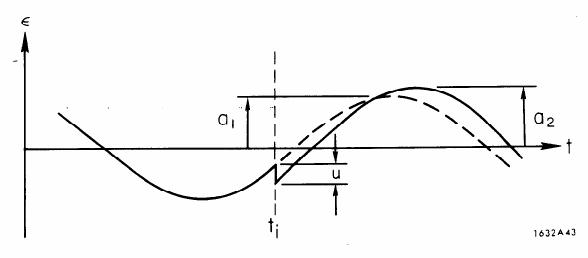
\includegraphics[width=0.8\linewidth]{./Figuras/fig43.jpeg}
	\caption{Effect on the energy oscillations of the emission of a quantum of energy $u$.}
	\label{fig:fig43}
\end{figure}
where\footnote{Obtained from $A^2 = \epsilon \epsilon^*$.}
\begin{align}
	A_1^2 = A_0^2 + u^2 - 2 A_0 u \cos \Omega (t_i - t_0),
\end{align}
and $t_1$ is some time displacement of no concern to us now. The quantum emission changes the amplitude of the oscillation to a new value which depends on the initial amplitude and on ($t_i - t_0$). Since the time $t_i$ at which a quantum emission occurs is completely unpredictable -- and since we are interested only in the cumulative affect of many such events -- we should ask only statistical questions. Such as: What is the probable amplitude change? In general, the phase ($t_i - t_0$) is completely random and the expectation value of $\cos\Omega(t_i - t_0)$ is therefore zero. Then, the probable amplitude change due to the quantum event is
\begin{align}\label{eq:5.25}
	\mean{\delta A^2} = \mean{A_1^2 - A_0^2} = \mean{u^2}
\end{align}
Notice that our result says that the probable change in $A^2$, which occurs when we add with random phase a new increment of oscillation of amplitude $u$, is just $u^2$ -- the same result we would have obtained for $\delta A^2$ if we had started with $A = 0$.\\
Suppose now that such quantum events occur in a random time sequence at the mean rate $\mathscr{N}$ (number per unit time). Each event changes $A^2$ by $u^2$; and since the mean time between events is $1/\mathscr{N}$, we expect that
\begin{align}\label{eq:5.26}
	\mean{\dfrac{dA^2}{dt}} = \mathscr{N} \mean{u^2}.
\end{align}
But the probable rate-of-change of $A^2$ is equal to the rate-of-change of the probable value of $A^2$ or
\begin{align} \label{eq:5.27}
	\dfrac{d}{dt}\mean{A^2} = \mathscr{N} \mean{u^2}.
\end{align}
In addition to exciting energy oscillations, the quantized energy losses contribute to a cumulative energy change. We have however, considered such average effects earlier. Their effect is to produce the energy oscillations as well as to cause the slow exponential damping of the amplitude $A$ with a time constant $\tau_\epsilon= 1/\alpha_\epsilon$. With such damping the amplitude decreases at the rate $A/\tau_\epsilon$; or its square at the rate $2A^2/\tau_\epsilon$. The probable amplitude must be similarly decreased by the damping which would contribute to the rate-of-change of $\mean{A^2}$ the amount
\begin{align} \label{eq:5.28}
	\dfrac{d}{dt}\mean{A^2} = -2 \dfrac{\mean{A^2}}{\tau_\epsilon}.
\end{align}
When both quantum excitation and damping are at work -- and other conditions are
stationary -- the rates of Eqs. \eqref{eq:5.27} and \eqref{eq:5.28} must sum to zero. We find that the probable value of $A^2$ is given by
\begin{align}
	\mean{A^2} = \dfrac{1}{2} \tau_\epsilon \mathscr{N} \mean{u^2}.
\end{align}
For the sinusoidal energy oscillations (as they are very nearly) the expectation value of $\epsilon$ is zero, and of its square -- which we shall call $\sigma_\epsilon^2$ -- is just $1/2$ the probable amplitude squared:
\begin{align}\label{eq:5.30}
	\sigma_\epsilon^2 = \mean{\epsilon^2} = \dfrac{\mean{A^2}}{2} = \dfrac{1}{4} \tau_\epsilon \mathscr{N} \mean{u^2}.
\end{align}
This then, would be the mean-square energy fluctuation in the energy oscillation which would be produced by the random emission of quanta.\\
An approximately equivalent result can be obtained from the following simple argument: The typical energy fluctuation comes from the deviation from its mean of the number of quanta emitted in one damping time $\tau_\epsilon$. The mean number emitted in $\tau_\epsilon$ is $\mathscr{N}\tau_\epsilon$, and so the rms deviation from the mean is $\sqrt{\mathscr{N}\tau_\epsilon}$ (Poisson distribution). Since each quantum has about the energy $u_c$, on the average,
\begin{align}
	\sigma_\epsilon = \sqrt{\mathscr{N}\tau_\epsilon} u_c.
\end{align}
The result is roughly the same as Eq.~\eqref{eq:5.30}. It is amusing to notice that, since $\mathscr{N} \approx P_\gamma/u_c$ and $\tau_\epsilon \approx E_0/P_\gamma$, we may also write that
\begin{align} \label{eq:5.32}
	\sigma_\epsilon \approx \sqrt{E_0 u_c}.
\end{align}
The energy fluctuation is roughly the geometric mean between the electron energy and the critical
 photon energy!\\
Let's now do a precise calculation which is somewhat more complicated -- first, because there is a distribution of quantum sizes and second, because both the distribution and the mean rate may vary around the storage ring. Returning to Eq.~\eqref{eq:5.28} we should consider separately the contribution to $d\mean{A^2}/dt$ from each interval of quantum sizes. Those quanta with energies between $u$ and $u + \Delta u$ -- of which there are $n(u)\Delta u$ - will give the contribution
\begin{align}
	\Delta \left\lbrace \dfrac{d}{dt}\mean{A^2} \right\rbrace = u^2 n(u) \Delta u.
\end{align}
But since the emission of quanta at the various different energies is also uncorrelated, each energy will contribute independently to the random-walk growth of $\mean{A^2}$. We need only sum the contributions from each interval $\Delta u$:
\begin{align}
	\dfrac{d}{dt}\mean{A^2} = \int_0^\infty u^2 n(u) du.
\end{align}
You will recognize the integral as just the product $\mathscr{N}\mean{u^2}$ considered in the preceding section -- Eq.~\eqref{eq:5.17}:
\begin{align}
	\dfrac{d}{dt} \mean{A^2} = \mathscr{N} \mean{u^2}.
\end{align}
The rate of growth just obtained depends on the electron energy -- which we may take to be the nominal energy $E_0$ -- and on $\rho$, the local radius of curvature of the trajectory, both of which may vary around the ring. From our derivation we may expect that the time for a ``significant'' change in the amplitude of the energy oscillation will be of the order of the damping time constant $\tau_\epsilon$. Since both the period of the oscillation $\approx 1/\Omega$,
 and the damping time $\tau_\epsilon$ are each much longer than a revolution time $T_0$ we may, without injustice, replace the rapidly varying quantity $\mathscr{N}\mean{u^2}$ by its mean value over one revolution of the ring. We shall also make a negligible error (on the average) if we replace the instantaneous radius of curvature $\rho$ of the trajectory at each azimuth $s$ by the local radius of curvature of the design orbit. Taking the average of $\mathscr{N}\mean{u^2}$
 over one revolution by integrating with respect to the azimuthal coordinate $s$, we may define\footnote{The index s on the brackets indicates that the average is taken over the coordinate $s$ as distinct from the average of $u^2$ which is over the distribution in $u$.},
\begin{align}
	Q_\epsilon = \mathscr{N}\mean{\mean{u^2}}_s = \dfrac{1}{L} \oint \mathscr{N} \mean{u^2} ds.
\end{align}
Following through the rest of the derivation as before we get for the mean-square energy fluctuation:
\begin{align} \label{eq:5.37}
	\sigma_\epsilon^2 = \dfrac{1}{4} \tau_\epsilon Q_\epsilon.
\end{align}
The simple form of our result is misleading; the complexities are hidden in $\tau_\epsilon$ and $Q_\epsilon$. Let's look first at $Q_\epsilon$. We need to evaluate $\mathscr{N} \mean{u^2}$ on the design orbit.\\
Suppose we begin with the form derived in Eq.~\eqref{eq:5.18}. $P_\gamma$ on the design orbit is
obtained from Eq.~\eqref{eq:4.4} by setting $E = E_0$ and $(1/\rho) = G$ (see Section~\ref{sec:2.2}), so
\begin{align}
	(P_\gamma)_\text{design orbit} = \dfrac{c C_\gamma}{2\pi} E_0^4 G^2,
\end{align}
which may be written -- using Eq.~\eqref{eq:4.9} -- as
\begin{align}
	(P_\gamma)_\text{design orbit} = \dfrac{\mean{P_\gamma}_s G^2}{\mean{G^2}_s}.
\end{align}
And $u_c$ on the design orbit is from Eq.~\eqref{eq:5.9},
\begin{align} \label{eq:5.40}
	(u_c)_\text{design orbit} = \dfrac{3}{2} \hslash c \gamma_0^3 |G|.
\end{align}
Then, we have that
\begin{align} \label{eq:5.41}
	\left( \mathscr{N} \mean{u^2} \right)_\text{design orbit} = C_u \dfrac{3}{2} \hslash c \gamma_0^3 |G| \dfrac{\mean{P_\gamma}_s G^2}{\mean{G^2}_s}
\end{align}
The only quantity which varies around the design orbit is $G$ so that $Q_\epsilon$, can be written as\footnote{We may now leave off the subscripts on the average since it is clear that all
quantities shown are to be averaged over $s$. I hope it is clear that $\mean{G^2}$, for example, means $\oint G^2(s)ds/L$ where $L$ is the orbit length.}
\begin{align}
	Q_\epsilon = \dfrac{3}{2} C_u \hslash c \gamma_0^3 P_\gamma \dfrac{\mean{|G|^3}}{\mean{G^2}}.
\end{align}
Taking $\tau_\epsilon$ from Eq.~\eqref{eq:4.53},
\begin{align}
	\tau_\epsilon = \dfrac{2E_0}{J_\epsilon \mean{P_\gamma}},
\end{align}
we may finally rewrite Eq.~\eqref{eq:5.37} as
\begin{align}
	\sigma_\epsilon^2 = \dfrac{3 C_u \hslash mc^3 \gamma_0^4 \mean{|G|^3}}{4 J_\epsilon \mean{G^2}}.
\end{align}
The relative energy spread $\sigma_\epsilon/E_0$ is usually more significant. We may write it as
\begin{align}\label{eq:5.45}
	\left(\dfrac{\sigma_\epsilon}{E_0}\right)^2 = \dfrac{C_q \gamma_0^2}{J_\epsilon} \dfrac{\mean{|G|^3}}{\mean{G^2}},
\end{align}
with $C_q$ -- which we may call the quantum constant -- given by
\begin{align} \label{eq:5.46}
	C_q = \dfrac{3 C_u \hslash}{4mc} = \dfrac{55}{32\sqrt{3}} \dfrac{\hslash}{mc} = 3.84 \times 10^{-13}\,\text{meter}.
\end{align}
It is very nearly, just the Compton wavelength of the electron.\\
The quantity $\mean{|G|^3}/J_\epsilon \mean{G^2}$ is a geometrical property of the guide field. Specifically,
\begin{align}
	\dfrac{\mean{|G|^3}}{J_\epsilon \mean{G^2}} = \dfrac{1}{J_\epsilon} \dfrac{\oint |G^3(s)|ds}{\oint G^2(s) ds}.
\end{align}
It is roughly equal to the inverse of the ``typical'' radius-of-curvature of the design orbit. The result of Eq.~\eqref{eq:5.45} is then roughly $\gamma^2$ times the ratio of the Compton wavelength to the orbit radius. For any ring the quantum induced spread in the relative energy deviation - namely $\sigma_\epsilon/E_0$ varies in direct proportion to the electron energy.\\
In a storage ring with an isomagnetic guide field (one which has a constant radius $\rho_0$ in the magnets and is straight elsewhere) the geometrical expression above is just $1/J_\epsilon \rho_0$, and
\begin{align}\label{eq:5.48}
	\left( \dfrac{\sigma_\epsilon}{E_0}\right)^2 = \dfrac{C_q \gamma_0^2}{J_\epsilon \rho_0}, && \text{(isomag.)}
\end{align}
In an isomagnetic storage ring with a 5 meter magnetic radius, electrons stored with an energy of 1 GeV will have an energy spread very nearly 0.04\% of the energy -- or about 40 keV.
